\chapter{NPIV Regression through Stochastic Approximate Gradients}

In this chapter, we present a novel approach to NPIV regression, which leverages stochastic approximate gradients to avoid computation of the adjoint operator $ \meanop^{ * } $.
The main idea is to search for $ h \in L^2 ( X ) $ which minimizes a certain risk measure $ \risk : L^2 ( X ) \to \R $.
The minimization is performed through an approximate SGD procedure, where $ h_{ m + 1 } = h_{ m } - \alpha_{ m } u_{ m } $ and $ u_{ m } $ is an approximate stochastic gradient for $ \risk $ at $ h_{ m } $.

\section{Risk measure}

Motivated by the fact that $ \hstar $ satisfies\footnote{Recall the notation introduced in the beginning of chapter \ref{chap: npiv and lip}.}
\begin{equation*}
    \meanop [ \hstar ] = r
,\end{equation*}
we introduce a pointwise loss function $ \ell : \R \times \R \to \R $ and define the \emph{populational risk measure} $ \risk : L^{ 2 } ( X ) \to \R $ associated with it to be
\begin{equation*}
    \risk ( h ) = \mean [ \ell ( r ( Z ), \meanop [ h ] ( Z ) ) ]
.\end{equation*}
Throughout the rest of this chapter, the example the reader should keep in mind is the quadratic\footnotemark~loss function $ \ell ( y, y' ) = \frac{ 1 }{ 2 } ( y - y' )^2 $.
\footnotetext{Although our results apply to more general loss functions, detailed experiments with setups in which other loss functions are more suitable are left for future work.}
Our goal is to solve the NPIV regression problem stated in subsection \ref{sec: problem specification} by solving
\begin{equation*}
    \inf_{ h \in \searchset } \risk ( h )
,\end{equation*}
where $ \searchset $ is a closed, convex, bounded subset of $ L^2 ( X ) $ such that $ (\hstar + \ker \meanop) \cap \searchset \neq \emptyset $.
This is a weaker condition than $ \hstar \in \searchset $, but which is sufficient for our theoretical results.
We also require $ 0 \in \searchset $.
For future reference, we state these conditions in
\begin{assump}[Regularity of $ \searchset $]
    \label{assumption on H}
    The set $ \searchset $ is a closed, convex, bounded subset of $ L^2 ( X ) $, which contains the origin and satisfies $ ( \hstar + \ker \meanop ) \cap \searchset \neq \emptyset $.
\end{assump}
The only part of this assumption which concerns the data generating process is $ ( \hstar + \ker \meanop ) \cap \searchset \neq \emptyset $.
This essentially means that the set $ \searchset $ is large enough so that there exists $ h \in \searchset $ to that $ \risk ( h ) = \risk ( \hstar ) $.
For $ \searchset $ satisfying assumption \ref{assumption on H}, we let $ D \defeq \diam \searchset < \infty $, so that $ \norm{ h } < D $ for every $ h \in \searchset $, since $ \norm{ h } = \norm{ h - 0 } < \diam \searchset $, as $ 0 \in \searchset $.
One possible choice for the set $ \searchset $ is the $ L^{ \infty } ( X ) $ ball contained in $ L^2 ( X ) $, that is
\begin{equation}
    \label{eq: H is L infinity ball}
    \searchset = \left\{ h \in L^2 ( X ) : \norm{ h }_{ \infty } < A \right\}
,\end{equation}
where $ A > 0 $ is a constant.
This set is obviously convex and bounded in the $ L^2 ( X ) $ norm.
It can be shown that it is also closed, but not necessarily compact, as can be seen by taking a $ \norm{ \cdot }_{ \infty } $--bounded orthonormal basis for $ L^2 ( X ) $, if one exists.
We denote by $ \pi_{ \searchset } $ the orthogonal projection onto $ \searchset $.
In case $ \searchset $ is given by (\ref{eq: H is L infinity ball}), we have the explicit formula:
\begin{equation*}
    \pi_{ \searchset } [ h ] = ( h^{ + } \wedge A ) - ( h^{ - } \wedge A )
.\end{equation*}

We now state all the assumptions needed on the pointwise loss $ \ell $.
We denote by $ \partial_{ 2 } $ a partial derivative with respect to the second argument.
\begin{assump}[Regularity of $ \ell $]
    \label{assumption loss}
    \begin{enumerate}
        \item[]
        \item The function $ \ell : \R \times \R \to \R $ is convex and $ C^2 $ with respect to its second argument;
        \item The function $ \ell $ has Lipschitz first derivative with respect to the second argument, i.e., there exists $ L \geq 0 $ such that, for all $ y, y', u, u' \in \R $ we have
            \begin{equation*}
                \abs{ \partial_{ 2 } \ell ( y, y' ) - \partial_{ 2 } \ell ( u, u' ) }
                \leq L ( \abs{ y - u } + \abs{ y' - u' } )
            .\end{equation*}
            \label{en: lipschitz gradients}
    \end{enumerate}
\end{assump}
Some useful facts which follow immediately from these assumptions are:
\begin{prop}
    \label{prop: loss properties}
    Assume that $ \ell $ satisfies Assumption \ref{assumption loss}.
    Then:
    \begin{enumerate}
        \item \label{bounded growth} Setting $ C_{ 0 } = \abs{ \partial_{ 2 } \ell ( 0, 0 ) } $ we have
            \begin{equation*}
                \abs{ \partial_{ 2 } \ell ( y, y' ) } \leq C_{ 0 } + L ( \abs{ y } + \abs{ y' } )
            \end{equation*}
            for all $ y, y' \in \R $;
        \item \label{continuous composition} The map $ f \mapsto \partial_{ 2 } \ell ( r_{ 0 } ( \cdot ), f ( \cdot ) ) $ from $ L^{ 2 } ( Z ) $ to $ L^{ 2 } ( Z ) $ is well-defined and $ L $-Lipschitz.
        \item \label{bounded second derivative} The second derivative with respect to the second argument is bounded: $ \abs{ \partial_{ 2 }^{ 2 } \ell ( y, y' ) } \leq L $ for all $ y, y' \in \R $;
    \end{enumerate}
\end{prop}
\begin{proof}
    \begin{enumerate}
        \item[]
        \item Write $ \partial_{ 2 } \ell ( y, y' ) = \partial_{ 2 } \ell ( y, y' ) - \partial_{ 2 } \ell ( 0, 0 ) + \partial_{ 2 } \ell ( 0, 0 ) $ and apply the triangle inequality as well as Assumption \ref{assumption loss}.\ref{en: lipschitz gradients}.
        \item From the previous item we know this map is well-defined.
            If $ f $ and $ g $ belong to $ L^{ 2 } ( Z ) $, we have
            \begin{align*}
                \norm{ \partial_{ 2 } \ell ( r_{ 0 } ( \cdot ), f ( \cdot ) ) - \partial_{ 2 } \ell ( r_{ 0 } ( \cdot ), g ( \cdot ) ) }_{ L^2 ( Z ) }^2
                &= \mean \left[
                    \abs{ 
                        \partial_{ 2 } ( r_{ 0 } ( Z ), f ( Z ) )
                        - \partial_{ 2 } ( r_{ 0 } ( Z ), g ( Z ) )
                    }^2
                \right] \\
                &\leq L^2 \mean \left[
                    \abs{ f ( Z ) - g ( Z ) }^2
                \right] \\
                &= L^2 \norm{ f - g }_{ L^2 ( Z ) }^2
            .\end{align*}
        \item Follows from the definition of derivative and Assumption \ref{assumption loss} \ref{en: lipschitz gradients}. \qedhere
    \end{enumerate}
\end{proof}

\section{Gradient computation}
As our strategy is based on minimizing the risk measure $ \risk $, we would like to compute an analytical formula for $ \nabla \risk ( h ) $, where $ h \in L^2 ( X ) $.
We start by computing the directional derivative of $ \risk $ at $ h $ in the direction $ f $, denoted by $ D \risk [ h ] ( f ) $:
\begin{align*}
    D \risk [ h ] ( f )
    &= \lim\limits_{ \delta \to 0 } \frac{ 1 }{ \delta } \left[
        \risk ( h + \delta f ) - \risk ( f )
    \right] \\
    &= \lim\limits_{ \delta \to 0 } \frac{ 1 }{ \delta } \mean \left[
        \ell ( r ( Z ), \meanop [ h + \delta f ] ( Z ) )
        -
        \ell ( r ( Z ), \meanop [ h ] ( Z ) )
    \right] \\
    &= \lim\limits_{ \delta \to 0 } \frac{ 1 }{ \delta } \mean \left[
        \ell ( r ( Z ), \meanop [ h ] ( Z ) + \delta \meanop [ f ] ( Z ) )
        -
        \ell ( r ( Z ), \meanop [ h ] ( Z ) )
    \right] \\
    \begin{split}
        &= \lim\limits_{ \delta \to 0 } \frac{ 1 }{ \delta } \mean \Biggl[
            \delta \partial_{ 2 } \ell ( r ( Z ), \meanop [ h ] ( Z ) ) \cdot \meanop [ f ] ( Z ) \\
        &\hspace{2cm}+ \frac{ \delta^2 }{ 2 } \partial_{ 2 }^2 \ell ( r ( Z ) , \meanop [ h + \theta f ] ( Z ) ) \cdot \meanop [ f ] ( Z )^2
        \Biggr]
    \end{split} \\
    \begin{split}
        &= \mean \left[
            \partial_{ 2 } \ell ( r ( Z ), \meanop [ h ] ( Z ) ) \cdot \meanop [ f ] ( Z )
        \right] \\
        &\hspace{2cm}+ \lim\limits_{ \delta \to 0 } \mean \Biggl[
            \frac{ \delta }{ 2 } \partial_{ 2 }^2 \ell ( r ( Z ) , \meanop [ h + \theta f ] ( Z ) ) \cdot \meanop [ f ] ( Z )^2
        \Biggr]
    \end{split} \\
    &= \mean \left[
        \partial_{ 2 } \ell ( r ( Z ), \meanop [ h ] ( Z ) ) \cdot \meanop [ f ] ( Z )
    \right]
,\end{align*}
where $ \theta \in ( 0, \delta ) $ is due to Taylor's formula.
The last step is then due to Proposition \ref{prop: loss properties} \ref{bounded second derivative}.
We can in fact expand the calculation a bit more, as follows:
\begin{align*}
    D \risk [ h ] ( f )
    &= \mean \left[
        \partial_{ 2 } \ell ( r ( Z ), \meanop [ h ] ( Z ) ) \cdot \meanop [ f ] ( Z )
    \right] \\
    &= \dotprod{ \partial_{ 2 } \ell ( r ( \cdot ), \meanop [ h ] ( \cdot ) ), \meanop [ f ] }_{ L^{ 2 } ( Z ) } \\
    &= \dotprod{ \meanop^{ * } [ \partial_{ 2 } \ell ( r ( Z ), \meanop [ h ] ( \cdot ) ) ], f }_{ L^{ 2 } ( X ) }
.\end{align*}
This shows that $ \risk $ is Gateux-differentiable, with Gateux derivative at $ h $ given by
\begin{equation*}
    D \risk [ h ] = \meanop^{ * } [ \partial_{ 2 } \ell ( r ( \cdot ), \meanop [ h ] ( \cdot ) ) ]
.\end{equation*}
By Proposition \ref{prop: loss properties} \ref{continuous composition} we have that $ h \mapsto D \risk [ h ] $ is a continuous mapping from $ L^{ 2 } ( X ) $ to $ L^{ 2 } ( X ) $, which implies that $ \risk $ is also Fréchet-differentiable, and both derivatives coincide \cite[Theorem~3.3]{pathak2018}.
Therefore,
\begin{equation}
    \label{eq: risk gradient}
   \nabla \risk ( h ) = \meanop^{ * } [ \partial_{ 2 } \ell ( r ( \cdot ), \meanop [ h ] ( \cdot ) ) ]  
.\end{equation}

Some previous approaches to NPIV, such as the one discussed in section \ref{sec: tikhonov}, involved approximating $ \meanop^{ * } $ directly using kernel methods.
We, in contrast, perform one more step before plugging in estimators.
From section \ref{sec: npiv and ill posed lip}, we know that $ \meanop^{ * } $ is an integral operator with kernel $ \Phi ( x, z ) = p_{ X, Z } ( x, z ) / ( p_{ X } ( x ) p_{ Z } ( z ) ) $, that is,
\begin{equation*}
    \meanop^{ * } [ g ] ( x ) = \mean [ \Phi ( x, Z ) g ( Z ) ] \quad \text{for all } g \in L^2 ( Z )
.\end{equation*}
Therefore, taking $ g ( z ) = \Phi ( x, z ) \partial_{ 2 } \ell ( r ( z ), \meanop [ h ] ( z ) ) $, we have that the random variable $ \Phi ( x, Z ) \partial_{ 2 } \ell ( r ( Z ), \meanop [ h ] ( Z ) ) $ is an unbiased stochastic estimate of $ \nabla \risk ( h ) ( x ) $.
In fact, a stronger result is true: we can consider $ \Phi ( \cdot, Z ) \partial_{ 2 } \ell ( r ( Z ), \meanop [ h ] ( Z ) ) $ as a random element of the Hilbert space $ L^2 ( X ) $, with mean vector --- in the Bochner integral sense, see \cite[Chapter~7]{hsing2015} --- equal to $ \nabla \risk ( h ) $.

A hypothesis which is needed for this proof and which is necessary for the following theoretical analysis is a finite $ L^2 ( \prob_{ X } \otimes \prob_{ Z } ) $--norm of $ \Phi $, which, as we have seen in section \ref{sec: npiv and ill posed lip}, amounts to saying $ \meanop $ is Hilbert-Schmidt.
\begin{assump}
    \label{assumption Phi}
    The kernel $ \Phi $ satisfies
    \begin{equation*}
        \norm{ \Phi }_{ L^2 ( \prob_{ X } \otimes \prob_{ Z } ) } \defeq \left( \int_{ \R^{ d_{ X } } \times \R^{ d_{ Z } } } \Phi ( x, z )^2 p_{ X } ( x ) p_{ Z } ( z ) \drm x \ddrm z \right)^{ \frac{ 1 }{ 2 } } < \infty
    .\end{equation*}
\end{assump}
This is the only restrictive assumption on the data generating process we have made so far, and, as we have discussed in section \ref{sec: npiv and ill posed lip}, it still allows the problem to be ill-posed.
This assumption is also present in the paper analyzed in section \ref{sec: tikhonov}.

\section{Stochastic Approximate Gradient Descent IV}

Our approximate stochastic gradient is then built using estimators $ \hat{ \Phi }, \hat{ r } $ and $ \hat{ \meanop } $ of $ \Phi, r $ and $ \meanop $ respectively.
With this notation, given a sample $ Z $ we have
\begin{equation}
    \label{eq: stochastic approximate gradient}
    \nabla \risk ( h ) ( x ) \approx \hat{ \Phi } ( x, Z ) \partial_{ 2 } \ell ( \hat{ r } ( Z ), \hat{ \meanop } [ h ] ( Z ) )
.\end{equation}
We remain agnostic to the specific ways in which $ \Phi, r $ and $ \meanop $ are being estimated.
All we require of these estimators is the following:
\begin{assump}[Properties of $ \hat{ \Phi }, \hat{ r } $ and $ \hat{ \meanop } $]
    \label{assumption estimators}
    \begin{enumerate}
        \item[] 
        \item $ \hat{ \Phi }, \hat{ r } $ and $ \hat{ \meanop } $ are computed using a dataset $ \dataset $ independent from the $ Z $ samples used in Algorithm \ref{algo: sagdiv}.
        \item $ \hat{ r } \in L^{ 2 } ( Z ) $ a.s.;
        \item $ \hat{ \meanop } : L^{ 2 } ( X ) \to L^{ 2 } ( Z ) $ is a bounded linear operator a.s., that is
            \begin{equation*}
                \norm{ \hat{ \meanop } }_{ \op } = \sup_{ \norm{ h }_{ L^2 ( X ) } = 1 } \norm{ \hat{ \meanop } [ h ] }_{ L^2 ( Z ) } < \infty
                \quad \text{a.s.}
            ;\end{equation*}
        \item $ \displaystyle \norm{ \hat{ \Phi } }_{ \infty } \defeq \sup_{
                \substack{
                x \in \R^{ d_{ X } } \\
                z \in \R^{ d_{ Z } }
            }
        } \abs{ \hat{ \Phi } ( x, z ) } < \infty $.
        This implies, in particular, that $ \norm{ \hat{ \Phi } }_{ L^2 ( \prob_{ X } \otimes \prob_{ Z } ) } < \infty $.
    \end{enumerate}
\end{assump}

We now present Stochastic Approximate Gradient Descent IV (SAGD--IV), an algorithm for estimating $ \hstar $ using the approximation given by (\ref{eq: stochastic approximate gradient}).

\begin{algorithm}[H]\label{algo: sagdiv}
    \caption{SAGD--IV}
    \SetKwInOut{Input}{input}
    \SetKwInOut{Output}{output}
    \Input{
        Samples $ \left\{ ( \bz_{ m } )_{ m=1 }^{ M } \right\} $.
        Estimators $ \hat{ \Phi }, \hat{ r } $ and $ \hat{ \meanop } $.
        Sequence of learning rates $ ( \alpha_{ m } )_{ m=1 }^{ M } $.
        Initial guess $ \hat{ h }_{ 0 } \in L^2 ( X ) $.
    }
    \Output{ $ \hat{ h } $ }
    \For{$ 1 \leq m \leq M $}{
    Set $ u_{ m } = \hat{ \Phi } ( \cdot , \bz_{ m } ) \partial_{ 2 } \ell \left( \hat{ r } ( \bz_{ m } ), \hat{ \meanop } [ \hat{ h }_{ m - 1 } ] ( \bz_{ m } ) \right) $ \;
    Set $ \hat{ h }_{ m }  = \pi_{ \searchset } \left[
        \hat{ h }_{ m-1 } - \alpha_{ m } u_{ m }  
    \right] $ \;
}
Set $ \hat{ h } = \frac{ 1 }{ M } \sum_{ m=1 }^{ M } \hat{ h }_{ m } $ \;
\end{algorithm}
We note the fact that the internal loop only needs samples from the instrumental variable $ Z $ to unfold.
This is due to the fact that our risk measure $ \risk $ directly compares $ r ( Z ) = \mean [ Y \mid Z ] $ and $ \meanop [ h ] ( Z ) $, instead of comparing $ \meanop [ h ] ( Z ) $ with $ Y $.
The drawback is that we have to estimate $ r $.

\section{Theoretical results}

\begin{rem}[Comment on notation]
    Let $ X $ and $ Y $ be arbitrary independent random variables.
    Then, given a function of two arguments $ f $, we have
    \begin{equation*}
        \mean [ f ( X, Y ) \mid Y ] = g ( Y )
    ,\end{equation*}
    where $ g ( y ) = \mean [ f ( X, y ) ] $.
    That is, to compute $ \mean [ f ( X, Y ) \mid Y ] $ we simply treat $ Y $ as constant and integrate in $ X $.
    We will denote this by writing $ \mean_{ X } [ f ( X, Y ) ] $.
\end{rem}

Since we are directly optimizing the risk measure, we are able to provide guarantees for $ \risk ( \hat{ h } ) $ in mean with respect to the training data $ \bz_{ 1:M } = \left\{ \bz_{ 1 }, \dots, \bz_{ m } \right\} $.
Our main result is the following, whose proof we present in the Appendix:
\begin{thm}
    \label{thm: main theorem}
    Let $ \hat{ h }_{ 0 }, \dots, \hat{ h }_{ M-1 } $ be generated according to Algorithm \ref{algo: sagdiv}.
    Assume that $ \ell $ satisfies Assumption \ref{assumption loss}, $ \searchset $ satisfies Assumption \ref{assumption on H}, $ \Phi $ satisfies Assumption \ref{assumption Phi} and $ \hat{ \Phi }, \hat{ r }, \hat{ \meanop } $ satisfy Assumption \ref{assumption estimators}.
    Then, if we let $ \hat{ h } = \sum_{ m=1 }^{ M } \hat{ h }_{ m-1 } $, the following bound holds:
    \begin{align}
        \begin{split}
            \mean_{ \bz_{ 1:M } } \left[
                \risk ( \hat{ h } ) - \risk ( \hstar )
            \right]
            &\leq \frac{ D^2 }{ 2 M \alpha_{ M } }
            + \frac{ \xi }{ M } \sum_{ m=1 }^{ M } \alpha_{ m } \\
            &\hspace{1cm}
            + \tau \cdot \left(
                \norm{ \Phi - \hat{ \Phi } }_{ L^{ 2 } ( \prob_{ X } \otimes \prob_{ Z } ) }^2 + \norm{ r - \hat{ r } }_{ L^2 ( Z ) }^2 + \norm{ \meanop - \hat{ \meanop } }_{ \op }^2
            \right)^{ \frac{ 1 }{ 2 } },
            \label{eq: main bound}
        \end{split}
    \end{align}
    where
    \begin{align*}
        \xi = \xi \left( \hat{ \Phi }, \hat{ r }, \hat{ \meanop } \right)
        &= \frac{ 3 }{ 2 } \norm{ \hat{ \Phi } }_{ \infty }^2 \left(
            C_{ 0 }^2 + L^2 \norm{ \hat{ r } }_{ L^2 ( Z ) }^2 + L^2 D ^2 \norm{ \hat{ \meanop } }_{ \op }^2
        \right), \\
        \tau = \tau \left( \hat{ \Phi } \right)
        &= 2 D \max \left\{
            3 ( C_{ 0 }^2 + L^2 \mean [ Y^2 ] + L^2 D^2 ),
            2L^2 \norm{ \hat{ \Phi } }_{ \infty }^2,
            2L^2 D^2 \norm{ \hat{ \Phi } }_{ \infty }^2
        \right\}
    .\end{align*}
\end{thm}

It is productive to analyze the RHS of the bound in (\ref{eq: main bound}) more carefully.
If we choose the sequence $ ( \alpha_{ m } ) $ to satisfy
\begin{equation*}
    M \alpha_{ M } \to \infty \quad \text{and} \quad \frac{ 1 }{ M } \sum_{ m=1 }^{ M } \alpha_{ m } \to 0
\end{equation*}
as $ M \to \infty $, then the first two terms in the sum vanish as $ M $ grows.
The last term is due to the fact that we do not know $ \Phi, r $ nor $ \meanop $, but it explicitly quantifies how the estimation errors of $ \hat{ \Phi }, \hat{ r } $ and $ \hat{ \meanop } $ come together to determine the quality of the final estimator.

\section{Computing the necessary estimators with kernel methods}
\label{sec: kernel methods}

In this section, we give references for how we chose to compute $ \hat{ \Phi }, \hat{ r } $ and $ \hat{ \meanop } $ in our practical implementation.
All of these estimators are based on kernel Ridge regression, where the unknown function is approximated using members of a Reproducing Kernel Hilbert Space (RKHS) --- see \cite[Chapter~4]{svm2008} for an introduction to these spaces. 
Kernel methods have the advantage of providing closed form solutions to regression problems due to the Representer Theorem \cite[Theorem~1]{representer2001}.

Starting with the estimator of
\begin{equation*}
    \Phi ( x, z ) = \frac{ p ( x, z ) }{ p ( x ) p ( z ) }
,\end{equation*}
we chose to use the Unconstrained Least Squares Importance Fitting (uLSIF) framework described in \cite[Chapter~6]{sugiyama2012}.
Using a gaussian kernel for the estimator, wee can see that it adheres to Assumption \ref{assumption estimators}.

The method of estimation of $ \hat{ \meanop } $ was taken to be the first stage of Kernel Instrumental Variable (KIV) \cite{singh2019}, a method for NPIV regression which provides two stages based on kernel Ridge regression.
The first stage consists of computing a conditional mean embedding \cite{cme2009} of the conditional distribution of $ X $ given $ Z = z $ in a RKHS of functions $ \mathcal{H}_{ \mathcal{X} } $, which acts as a proxy for $ L^2 ( X ) $.
This conditional mean embedding encodes the same information as $ \meanop $.
To estimate $ r ( Z ) = \mean [ Y \mid Z ] $, we simply used this same method to obtain an approximation to the operator $ L^2 ( Y ) : f \mapsto \mean [ f ( Y ) \mid Z = \cdot \ ] \in L^2 ( Z ) $, which we then apply to the identity function.

\section{Numerical experiment}

We tested SAGD-IV using the following data generating process, obtained from \cite{deepgmm2019}:

\begin{tabular}{lcl}
    $ Y = \hstar ( X ) + \varepsilon + \delta $ & &
    $ X = Z_{ 1 } + \varepsilon + \gamma $ \\
    $ Z = ( Z_{ 1 }, Z_{ 2 } ) \sim \unif ( [-3, 3]^2 ) $ & &
    $ \varepsilon \sim \mathcal{N} ( 0, 1 ), \ \gamma, \delta \sim \mathcal{N} ( 0, 0.1 ) $
\end{tabular}

\noindent For the response function $ \hstar $, we tested two cases:
\begin{equation*}
    \bsin: \hstar ( x ) = \sin ( x ) \quad \text{and} \quad \babs: \hstar ( x ) = \abs{ x }
.\end{equation*}
We chose to compare our model to a direct competitor: Kernel Instrumental Variable (KIV) \cite{singh2019}, due to the relationship between both methods discussed in section \ref{sec: kernel methods}.
All regularization parameters necessary for the computation of $ \hat{ \Phi }, \hat{ r }, \hat{ \meanop } $, as well as the ones in the two stages of KIV, were chosen using cross-validation on held-out training samples.
All kernels employed were gaussian, with lenghtscale parameter set to be equal to the inverse of the median distance between samples.
With the notation of Algorithm \ref{algo: sagdiv}, for SAGD-IV we set the learning rate to be $ \alpha_{ m } = \frac{ 1 }{ \sqrt{ M } } $ for $ 1 \leq m \leq M $.
For SAGD-IV, the dataset was comprised of $ 600 $ samples from the triple $ ( X, Z, Y ) $ and an additional $ 1200 $ samples of $ Z $ alone, to conduct the loop in Algorithm \ref{algo: sagdiv}.
The dataset for KIV was comprised of the same $ 600 $ samples of the triple $ ( X, Z, Y ) $, plus additional $ 600 $ samples of the pair $ ( Z, Y ) $ (these are necessary for the algorithm, see \cite{singh2019}).
In this way, both algorithms have access to the same amount of samples and share as many as possible.

The results obtained are in Figure \ref{fig: sagd-iv and kiv}.
\begin{figure}[htb]
    \begin{center}
        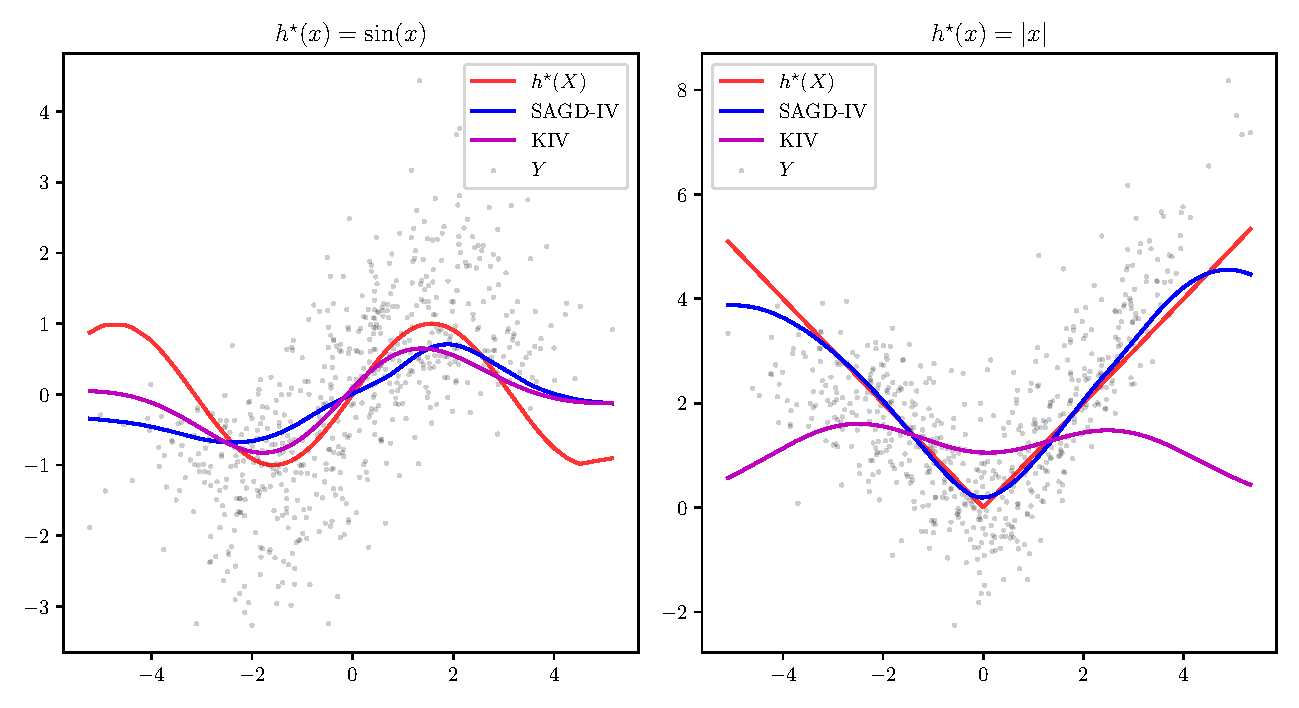
\includegraphics[width=\textwidth]{sagd-iv_kiv_comparison.pdf}
    \end{center}
    \caption{
    SAGD-IV and KIV for two different response functions.
}
    \label{fig: sagd-iv and kiv}
\end{figure}
We can see that, while both methods performed similarly in the $ \bsin $ case, KIV was slightly better.
This might be due to the smooth nature of the KIV estimator, since both stages are conducted using Kernel Ridge Regression.
However, the relative performance changes drastically when looking at the $ \babs $ case, where SAGD-IV greatly outperformed KIV.
This indicates that SAGD-IV may perform better with non-smooth response functions.
Of course, this isn't a thorough investigation of the empirical performance of SAGD-IV, nor irrefutable proof that it is better then KIV, and a more detailed analysis, involving other recent methods which have appeared in the NPIV literature, is left for future work.
